\documentclass[
    language=english,
    doctype=article,
    institution=none,
    titlestyle=book,
]{../../omnilatex}

\RequirePackage{config/document-settings}
\addbibresource{../../bib/bibliography.bib}

\RequirePackage{tikz}
\RequirePackage{pgfplots}
\pgfplotsset{compat=1.18}
\usetikzlibrary{
    arrows.meta,
    positioning,
    shapes.geometric,
    shapes,
    calc,
    fit,
    backgrounds,
    decorations.pathreplacing,
    decorations.pathmorphing,
    patterns,
    matrix,
    shadows,
    trees,
    mindmap,
    chains,
    quotes,
    angles,
    babel,
}
\usepgfplotslibrary{groupplots,patchplots,colorbrewer}
\RequirePackage{circuitikz}
\RequirePackage{pgf-pie}
\RequirePackage{booktabs}
\RequirePackage{subcaption}
\RequirePackage{float}

\begin{document}

\maketitle

\begin{abstract}
This gallery showcases 22 distinct TikZ and pgfplots diagram types commonly used
in scientific publications, technical documentation, and presentations. Each example
is self-contained with annotations explaining key techniques.
\end{abstract}

\tableofcontents

% =====================================================
\section{Flowchart}
\label{sec:flowchart}
% =====================================================

A process flowchart with decision diamonds and parallel paths.

\begin{figure}[htbp]
    \centering
    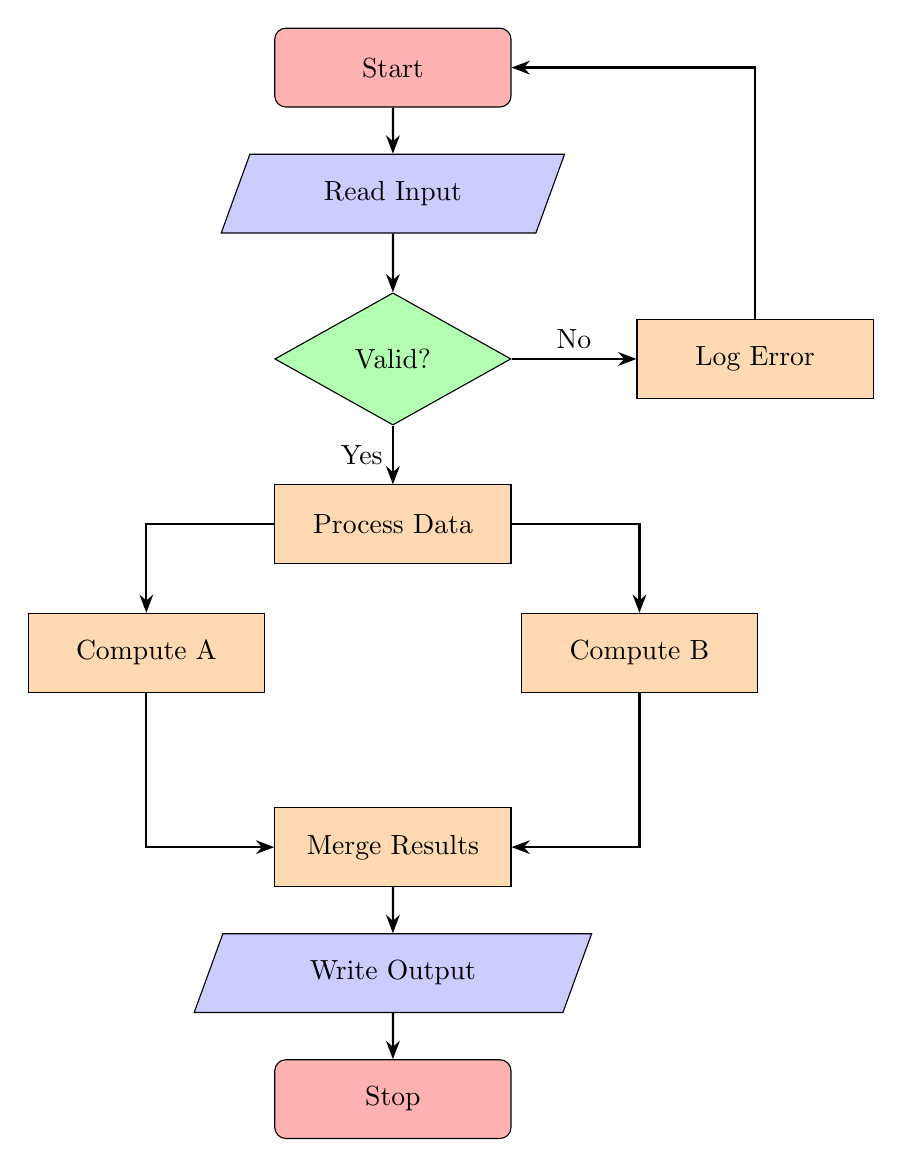
\begin{tikzpicture}[
        node distance=1.6cm and 2cm,
        startstop/.style={rectangle, rounded corners, minimum width=3cm,
            minimum height=1cm, text centered, draw=black, fill=red!30},
        process/.style={rectangle, minimum width=3cm, minimum height=1cm,
            text centered, draw=black, fill=orange!30},
        decision/.style={diamond, minimum width=3cm, minimum height=1cm,
            text centered, draw=black, fill=green!30},
        io/.style={trapezium, trapezium left angle=70, trapezium right angle=110,
            minimum width=3cm, minimum height=1cm, text centered, draw=black, fill=blue!20},
        arrow/.style={thick, ->, >=Stealth},
    ]
        \node (start) [startstop] {Start};
        \node (input) [io, below of=start] {Read Input};
        \node (validate) [decision, below of=input, yshift=-0.5cm] {Valid?};
        \node (error) [process, right of=validate, xshift=3cm] {Log Error};
        \node (process1) [process, below of=validate, yshift=-0.5cm] {Process Data};
        \node (parallel1) [process, below left of=process1, xshift=-2cm, yshift=-0.5cm] {Compute A};
        \node (parallel2) [process, below right of=process1, xshift=2cm, yshift=-0.5cm] {Compute B};
        \node (merge) [process, below of=process1, yshift=-2.5cm] {Merge Results};
        \node (output) [io, below of=merge] {Write Output};
        \node (stop) [startstop, below of=output] {Stop};

        \draw [arrow] (start) -- (input);
        \draw [arrow] (input) -- (validate);
        \draw [arrow] (validate) -- node[anchor=south] {No} (error);
        \draw [arrow] (validate) -- node[anchor=east] {Yes} (process1);
        \draw [arrow] (process1) -| (parallel1);
        \draw [arrow] (process1) -| (parallel2);
        \draw [arrow] (parallel1) |- (merge);
        \draw [arrow] (parallel2) |- (merge);
        \draw [arrow] (merge) -- (output);
        \draw [arrow] (output) -- (stop);
        \draw [arrow] (error) |- (start);
    \end{tikzpicture}
    \caption{Flowchart with decision branching and parallel processing paths.}
    \label{fig:flowchart}
\end{figure}

% =====================================================
\section{Neural Network}
\label{sec:neural-network}
% =====================================================

A multi-layer feed-forward neural network with weighted connections.

\begin{figure}[htbp]
    \centering
    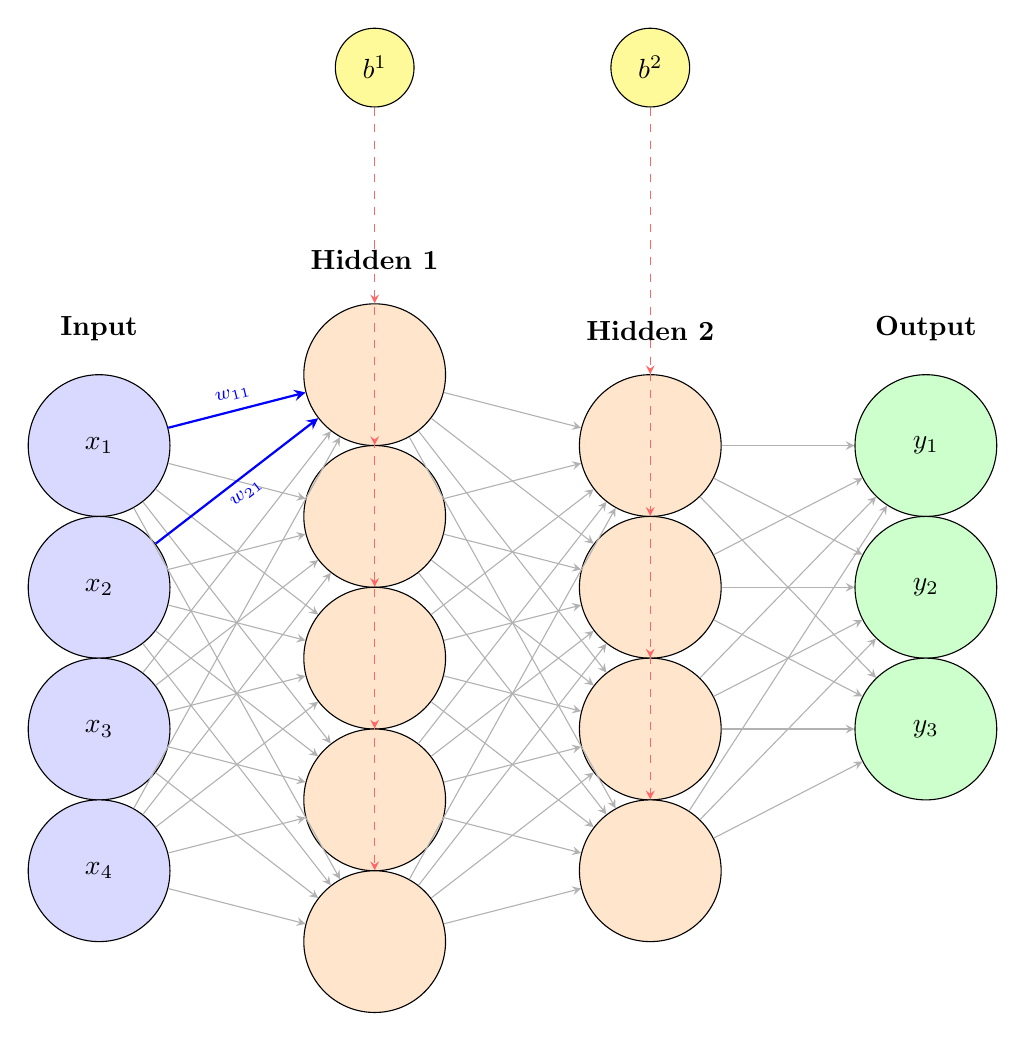
\begin{tikzpicture}[
        neuron/.style={circle, draw=black, fill=white, minimum size=18mm, inner sep=0pt},
        input-neuron/.style={neuron, fill=blue!15},
        hidden-neuron/.style={neuron, fill=orange!20},
        output-neuron/.style={neuron, fill=green!20},
        connection/.style={->, >=stealth, thin},
        bias/.style={circle, draw=black, fill=yellow!40, minimum size=10mm, inner sep=0pt},
    ]
        % Input layer
        \foreach \i in {1,...,4} {
            \node[input-neuron] (I\i) at (0, -\i*1.8) {$x_{\i}$};
        }
        % Hidden layer 1
        \foreach \j in {1,...,5} {
            \node[hidden-neuron] (H1\j) at (3.5, -\j*1.8 + 0.9) {};
        }
        % Hidden layer 2
        \foreach \j in {1,...,4} {
            \node[hidden-neuron] (H2\j) at (7, -\j*1.8 + 0) {};
        }
        % Output layer
        \foreach \k in {1,...,3} {
            \node[output-neuron] (O\k) at (10.5, -\k*1.8 + 0) {$y_{\k}$};
        }
        % Bias nodes
        \node[bias] (b1) at (3.5, 3) {$b^1$};
        \node[bias] (b2) at (7, 3) {$b^2$};

        % Input to Hidden 1 connections
        \foreach \i in {1,...,4}
            \foreach \j in {1,...,5}
                \draw[connection, gray!60] (I\i) -- (H1\j);

        % Hidden 1 to Hidden 2 connections
        \foreach \j in {1,...,5}
            \foreach \k in {1,...,4}
                \draw[connection, gray!60] (H1\j) -- (H2\k);

        % Hidden 2 to Output connections
        \foreach \j in {1,...,4}
            \foreach \k in {1,...,3}
                \draw[connection, gray!60] (H2\j) -- (O\k);

        % Bias connections
        \foreach \j in {1,...,5}
            \draw[connection, dashed, red!60] (b1) -- (H1\j);
        \foreach \j in {1,...,4}
            \draw[connection, dashed, red!60] (b2) -- (H2\j);

        % Layer labels
        \node[above=0.3cm of I1, font=\bfseries] {Input};
        \node[above=0.3cm of H11, font=\bfseries] {Hidden 1};
        \node[above=0.3cm of H21, font=\bfseries] {Hidden 2};
        \node[above=0.3cm of O1, font=\bfseries] {Output};

        % Weight annotations on select connections
        \draw[connection, blue, thick] (I1) -- node[above, sloped, font=\scriptsize] {$w_{11}$} (H11);
        \draw[connection, blue, thick] (I2) -- node[below, sloped, font=\scriptsize] {$w_{21}$} (H11);
    \end{tikzpicture}
    \caption{Multi-layer neural network with two hidden layers, bias nodes, and weighted connections.}
    \label{fig:neural-network}
\end{figure}

% =====================================================
\section{State Diagram}
\label{sec:state-diagram}
% =====================================================

A finite automaton with labeled state transitions.

\begin{figure}[htbp]
    \centering
    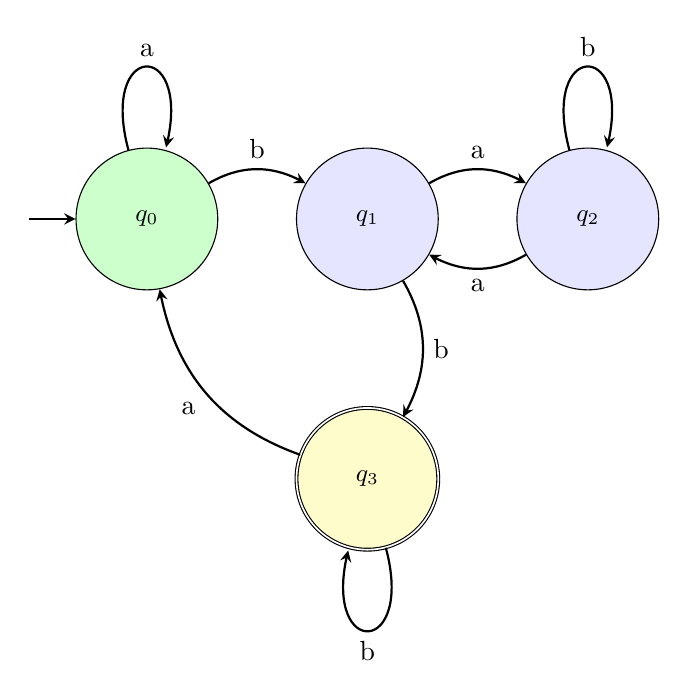
\begin{tikzpicture}[
        state/.style={circle, draw=black, fill=blue!10, minimum size=18mm,
            inner sep=0pt, font=\small},
        initial/.style={state, fill=green!20},
        accept/.style={state, double, fill=yellow!20},
        every edge/.style={draw, ->, >=stealth, thick},
        auto, node distance=2.8cm,
    ]
        \node[initial] (q0) {$q_0$};
        \node[state] (q1) [right of=q0] {$q_1$};
        \node[state] (q2) [right of=q1] {$q_2$};
        \node[accept] (q3) [below of=q1, yshift=-0.5cm] {$q_3$};

        \path
            (q0) edge [loop above] node {a} (q0)
            (q0) edge [bend left] node {b} (q1)
            (q1) edge [bend left] node {a} (q2)
            (q1) edge [bend left] node {b} (q3)
            (q2) edge [bend left] node {a} (q1)
            (q2) edge [loop above] node {b} (q2)
            (q3) edge [bend left] node {a} (q0)
            (q3) edge [loop below] node {b} (q3);

        % Start arrow
        \draw[->, >=stealth, thick] (-1.5, 0) -- (q0);
    \end{tikzpicture}
    \caption{Finite automaton accepting strings ending with ``ab''. Double circle marks the accepting state.}
    \label{fig:state-diagram}
\end{figure}

% =====================================================
\section{Network Graph}
\label{sec:network-graph}
% =====================================================

A computer network topology with labeled nodes and weighted edges.

\begin{figure}[htbp]
    \centering
    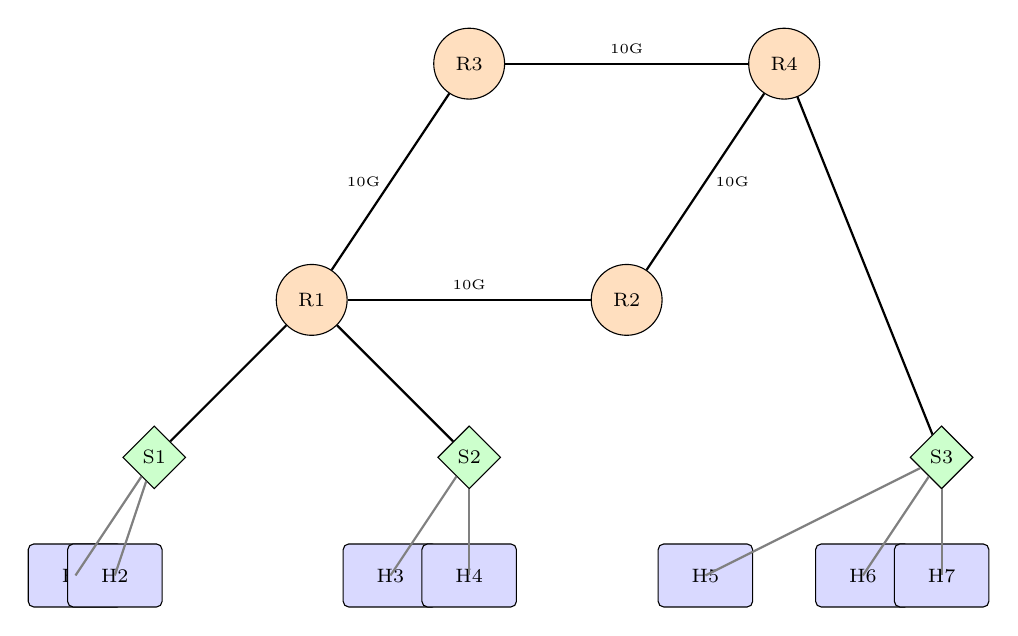
\begin{tikzpicture}[
        host/.style={rectangle, draw, fill=blue!15, minimum width=1.2cm,
            minimum height=0.8cm, font=\scriptsize, rounded corners=2pt},
        router/.style={circle, draw, fill=orange!25, minimum size=0.9cm,
            font=\scriptsize},
        switch/.style={diamond, draw, fill=green!20, minimum size=0.8cm,
            font=\scriptsize, inner sep=1pt},
        link/.style={thick, -},
    ]
        % Core routers
        \node[router] (r1) at (0,0) {R1};
        \node[router] (r2) at (4,0) {R2};
        \node[router] (r3) at (2,3) {R3};
        \node[router] (r4) at (6,3) {R4};

        % Switches
        \node[switch] (s1) at (-2,-2) {S1};
        \node[switch] (s2) at (2,-2) {S2};
        \node[switch] (s3) at (8,-2) {S3};

        % Hosts
        \foreach \x/\label in {-3/H1, -2.5/H2} {
            \node[host] at (\x, -3.5) {\label};
        }
        \node[host] at (1, -3.5) {H3};
        \node[host] at (2, -3.5) {H4};
        \node[host] at (5, -3.5) {H5};
        \node[host] at (7, -3.5) {H6};
        \node[host] at (8, -3.5) {H7};

        % Core links
        \draw[link] (r1) -- node[above, font=\tiny] {10G} (r2);
        \draw[link] (r1) -- node[left, font=\tiny] {10G} (r3);
        \draw[link] (r3) -- node[above, font=\tiny] {10G} (r4);
        \draw[link] (r2) -- node[right, font=\tiny] {10G} (r4);

        % Access links
        \draw[link] (r1) -- (s1);
        \draw[link] (r1) -- (s2);
        \draw[link] (r4) -- (s3);

        % Host links
        \draw[link, gray] (s1) -- (-3, -3.5);
        \draw[link, gray] (s1) -- (-2.5, -3.5);
        \draw[link, gray] (s2) -- (1, -3.5);
        \draw[link, gray] (s2) -- (2, -3.5);
        \draw[link, gray] (s3) -- (5, -3.5);
        \draw[link, gray] (s3) -- (7, -3.5);
        \draw[link, gray] (s3) -- (8, -3.5);
    \end{tikzpicture}
    \caption{Network topology with routers (circles), switches (diamonds), and hosts (rectangles).}
    \label{fig:network-graph}
\end{figure}

% =====================================================
\section{Tree Diagram}
\label{sec:tree}
% =====================================================

A hierarchical tree with recursive branching.

\begin{figure}[htbp]
    \centering
    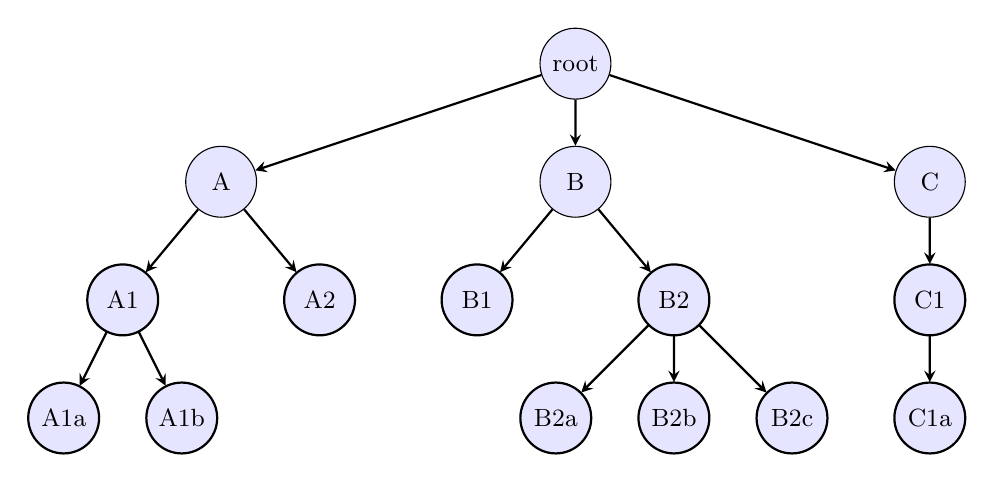
\begin{tikzpicture}[
        level 1/.style={sibling distance=4.5cm},
        level 2/.style={sibling distance=2.5cm},
        level 3/.style={sibling distance=1.5cm},
        every node/.style={draw, circle, fill=blue!10, minimum size=9mm,
            font=\small, inner sep=0pt},
        edge from parent/.style={draw, ->, >=stealth, thick},
        grow=down,
    ]
        \node {root}
            child { node {A}
                child { node {A1}
                    child { node {A1a} }
                    child { node {A1b} }
                }
                child { node {A2} }
            }
            child { node {B}
                child { node {B1} }
                child { node {B2}
                    child { node {B2a} }
                    child { node {B2b} }
                    child { node {B2c} }
                }
            }
            child { node {C}
                child { node {C1}
                    child { node {C1a} }
                }
            };
    \end{tikzpicture}
    \caption{Hierarchical tree with three levels of branching.}
    \label{fig:tree}
\end{figure}

% =====================================================
\section{Venn Diagram}
\label{sec:venn}
% =====================================================

Overlapping sets visualized with a three-set Venn diagram.

\begin{figure}[htbp]
    \centering
    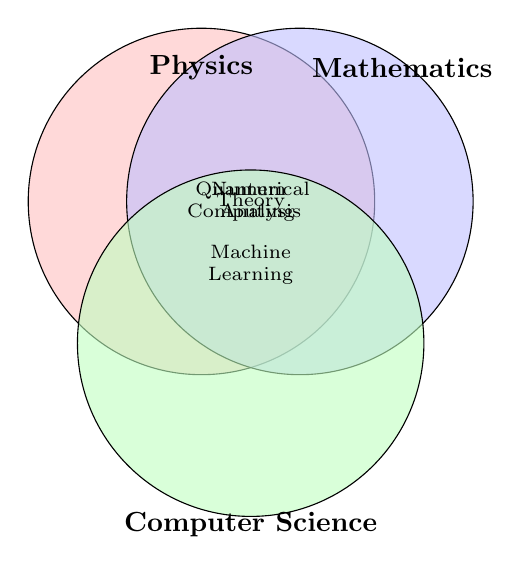
\begin{tikzpicture}
        \def\radius{2.2}
        \def\cx{1.5}
        \def\cy{-1.8}

        \draw[fill=red!25, fill opacity=0.6] (\cx, \cy + 1.3) circle (\radius);
        \draw[fill=blue!25, fill opacity=0.6] (\cx + \cx/1.2, \cy + 1.3) circle (\radius);
        \draw[fill=green!25, fill opacity=0.6] (\cx + \cx/2.4, \cy - 0.5) circle (\radius);

        \node at (\cx, \cy + 3.0) {\textbf{Physics}};
        \node at (\cx + \cx/1.2 + 1.3, \cy + 3.0) {\textbf{Mathematics}};
        \node at (\cx + \cx/2.4, \cy - 2.8) {\textbf{Computer Science}};

        % Intersection labels
        \node[font=\scriptsize, text width=2cm, align=center] at (\cx + 0.5, \cy + 1.3) {Quantum Computing};
        \node[font=\scriptsize, text width=2cm, align=center] at (\cx + \cx/1.2 - 0.5, \cy + 1.3) {Numerical Analysis};
        \node[font=\scriptsize, text width=2cm, align=center] at (\cx + \cx/2.4, \cy + 0.5) {Machine Learning};
        \node[font=\scriptsize, text width=2cm, align=center] at (\cx + \cx/2.4, \cy + 1.3) {Theory};
    \end{tikzpicture}
    \caption{Three-set Venn diagram showing interdisciplinary overlaps.}
    \label{fig:venn}
\end{figure}

% =====================================================
\section{Pie Chart}
\label{sec:pie}
% =====================================================

A hand-drawn-style pie chart using the \texttt{pgf-pie} package.

\begin{figure}[htbp]
    \centering
    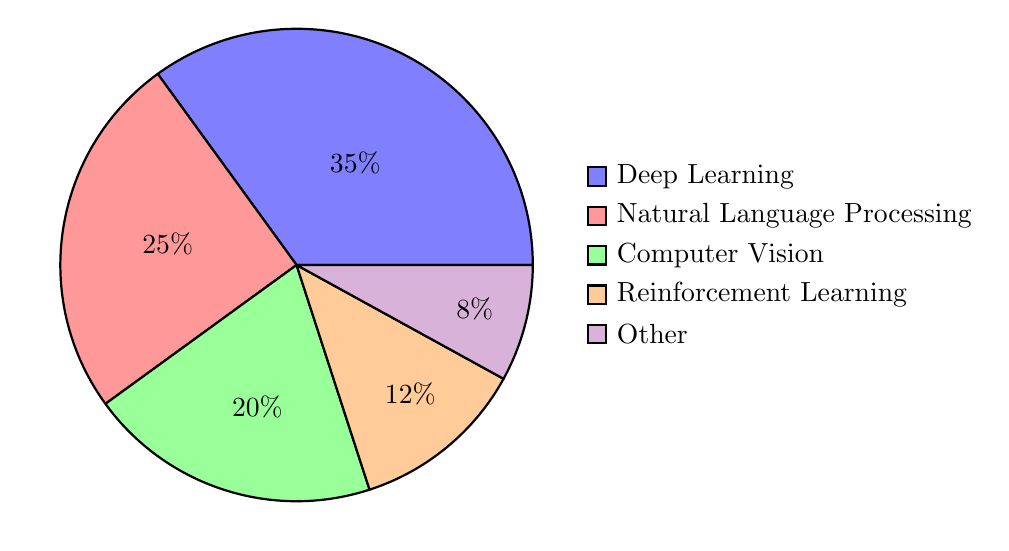
\begin{tikzpicture}
        \pie[
            text=legend,
            radius=3,
            color={blue!50, red!40, green!40, orange!40, violet!30},
            before number=\phantom{0},
            after number=\%,
        ]{
            35/Deep Learning,
            25/Natural Language Processing,
            20/Computer Vision,
            12/Reinforcement Learning,
            8/Other
        }
    \end{tikzpicture}
    \caption{Research area distribution in modern AI (2026).}
    \label{fig:pie}
\end{figure}

% =====================================================
\section{Grouped Bar Chart}
\label{sec:bar-chart}
% =====================================================

A grouped bar chart comparing metrics across categories.

\begin{figure}[htbp]
    \centering
    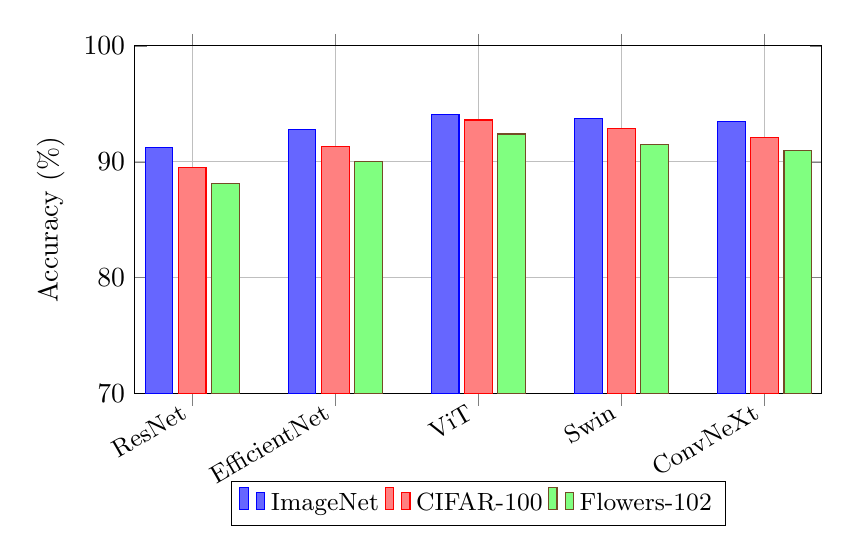
\begin{tikzpicture}
    \begin{axis}[
        ybar,
        bar width=10pt,
        width=0.85\textwidth,
        height=6cm,
        ylabel={Accuracy (\%)},
        symbolic x coords={ResNet, EfficientNet, ViT, Swin, ConvNeXt},
        xtick=data,
        x tick label style={rotate=30, anchor=east, font=\small},
        ymin=70, ymax=100,
        legend style={at={(0.5,-0.25)}, anchor=north, legend columns=3,
            font=\small},
        grid=major,
        every node near coord/.append style={font=\tiny, rotate=90, anchor=west},
    ]
        \addplot+[fill=blue!60] coordinates {
            (ResNet,91.2) (EfficientNet,92.8) (ViT,94.1) (Swin,93.7) (ConvNeXt,93.5)
        };
        \addplot+[fill=red!50] coordinates {
            (ResNet,89.5) (EfficientNet,91.3) (ViT,93.6) (Swin,92.9) (ConvNeXt,92.1)
        };
        \addplot+[fill=green!50] coordinates {
            (ResNet,88.1) (EfficientNet,90.0) (ViT,92.4) (Swin,91.5) (ConvNeXt,91.0)
        };
        \legend{ImageNet, CIFAR-100, Flowers-102}
    \end{axis}
    \end{tikzpicture}
    \caption{Classification accuracy of five architectures across three datasets.}
    \label{fig:bar-chart}
\end{figure}

% =====================================================
\section{Line Plot with Legend}
\label{sec:line-plot}
% =====================================================

Multiple lines showing training loss curves.

\begin{figure}[htbp]
    \centering
    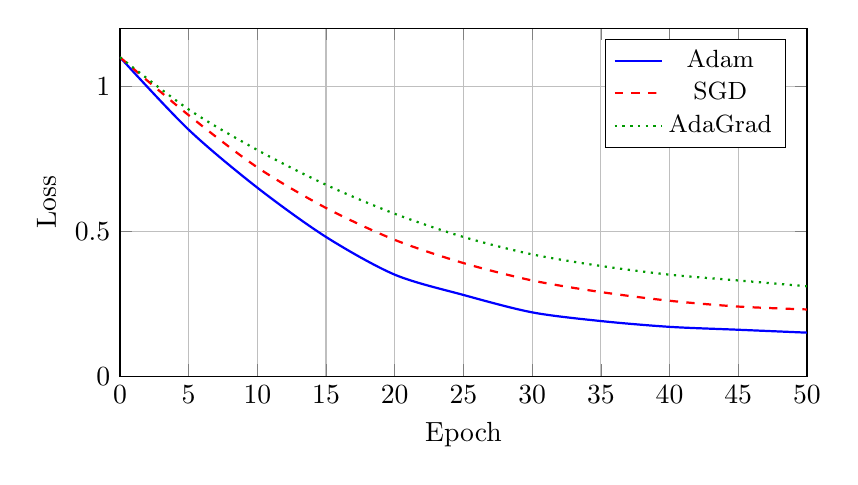
\begin{tikzpicture}
    \begin{axis}[
        width=0.85\textwidth,
        height=6cm,
        xlabel={Epoch},
        ylabel={Loss},
        grid=major,
        legend pos=north east,
        legend style={font=\small},
        xmin=0, xmax=50,
        ymin=0, ymax=1.2,
    ]
        \addplot[color=blue, thick, smooth] coordinates {
            (0,1.1) (5,0.85) (10,0.65) (15,0.48) (20,0.35)
            (25,0.28) (30,0.22) (35,0.19) (40,0.17) (45,0.16) (50,0.15)
        };
        \addplot[color=red, thick, smooth, dashed] coordinates {
            (0,1.1) (5,0.9) (10,0.72) (15,0.58) (20,0.47)
            (25,0.39) (30,0.33) (35,0.29) (40,0.26) (45,0.24) (50,0.23)
        };
        \addplot[color=green!60!black, thick, smooth, dotted] coordinates {
            (0,1.1) (5,0.92) (10,0.78) (15,0.66) (20,0.56)
            (25,0.48) (30,0.42) (35,0.38) (40,0.35) (45,0.33) (50,0.31)
        };
        \legend{Adam, SGD, AdaGrad}
    \end{axis}
    \end{tikzpicture}
    \caption{Training loss convergence for three optimizers.}
    \label{fig:line-plot}
\end{figure}

% =====================================================
\section{Scatter Plot with Trend Line}
\label{sec:scatter}
% =====================================================

Scatter plot with a linear regression trend line.

\begin{figure}[htbp]
    \centering
    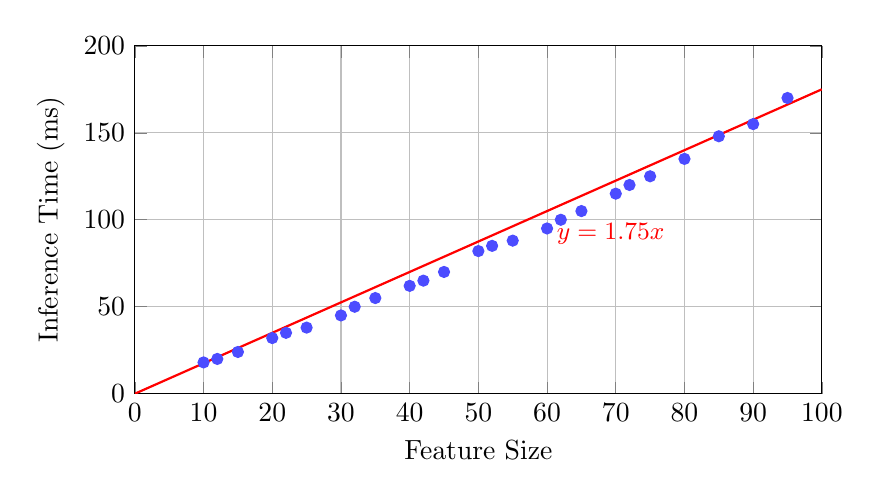
\begin{tikzpicture}
    \begin{axis}[
        width=0.85\textwidth,
        height=6cm,
        xlabel={Feature Size},
        ylabel={Inference Time (ms)},
        grid=major,
        xmin=0, xmax=100,
        ymin=0, ymax=200,
    ]
        \addplot[only marks, mark=*, mark size=2pt, blue!70] coordinates {
            (10,18) (15,24) (20,32) (25,38) (30,45)
            (35,55) (40,62) (45,70) (50,82) (55,88)
            (60,95) (65,105) (70,115) (75,125) (80,135)
            (85,148) (90,155) (95,170) (12,20) (22,35)
            (32,50) (42,65) (52,85) (62,100) (72,120)
        };
        % Trend line: y = 1.75x
        \addplot[red, thick, domain=0:100, samples=2] {1.75*x};
        \node[red, anchor=south west] at (axis cs:60,80) {\small $y = 1.75x$};
    \end{axis}
    \end{tikzpicture}
    \caption{Scatter plot of feature size vs.\ inference time with linear trend line.}
    \label{fig:scatter}
\end{figure}

% =====================================================
\section{Heatmap}
\label{sec:heatmap}
% =====================================================

A matrix heatmap with color-coded correlation values.

\begin{figure}[htbp]
    \centering
    \begin{tikzpicture}
        \def\n{6}
        \def\cellsize{0.9}
        \pgfmathsetseed{42}

        % Correlation matrix data (symmetric)
        \def\corrA{1.0, 0.8, 0.3, -0.1, 0.5, 0.2}
        \def\corrB{0.8, 1.0, 0.5, 0.0, 0.6, 0.3}
        \def\corrC{0.3, 0.5, 1.0, 0.7, 0.4, 0.6}
        \def\corrD{-0.1, 0.0, 0.7, 1.0, 0.2, 0.8}
        \def\corrE{0.5, 0.6, 0.4, 0.2, 1.0, 0.5}
        \def\corrF{0.2, 0.3, 0.6, 0.8, 0.5, 1.0}

        \foreach \row/\data/\y in {
            1/\corrA/0, 2/\corrB/-1, 3/\corrC/-2,
            4/\corrD/-3, 5/\corrE/-4, 6/\corrF/-5
        } {
            \foreach \val [count=\i from 0] in \data {
                \pgfmathparse{\val}
                \pgfmathsetmacro{\intensity}{abs(\pgfmathresult)}
                \pgfmathtruncatemacro{\sign}{\pgfmathresult > 0 ? 1 : 0}
                \pgfmathtruncatemacro{\ri}{255}
                \pgfmathtruncatemacro{\gi}{round(255*(1-\intensity))}
                \pgfmathtruncatemacro{\bi}{round(255*(1-\intensity))}
                \ifnum \sign > 0
                    \definecolor{cellcolor}{RGB}{\ri,\gi,\bi}
                \else
                    \definecolor{cellcolor}{RGB}{\gi,\bi,\ri}
                \fi
                \fill[cellcolor] (\i*\cellsize, \y*\cellsize) rectangle
                    ++(\cellsize, \cellsize);
                \node[font=\scriptsize] at (\i*\cellsize + 0.45, \y*\cellsize + 0.45)
                    {\pgfmathprintnumber[precision=1]{\pgfmathresult}};
            }
        }

        % Labels
        \foreach \label/\x in {A/0, B/1, C/2, D/3, E/4, F/5} {
            \node[font=\small, below] at (\x*\cellsize + 0.45, -5.5*\cellsize) {\label};
            \node[font=\small, left] at (-0.2, -\x*\cellsize + 0.45) {\label};
        }

        % Title
        \node[font=\bfseries] at (2.7, 1) {Correlation Matrix};
    \end{tikzpicture}
    \caption{Correlation heatmap between six features. Red indicates positive, blue indicates negative correlation.}
    \label{fig:heatmap}
\end{figure}

% =====================================================
\section{Contour Plot}
\label{sec:contour}
% =====================================================

An elevation-map style contour plot using pgfplots.

\begin{figure}[htbp]
    \centering
    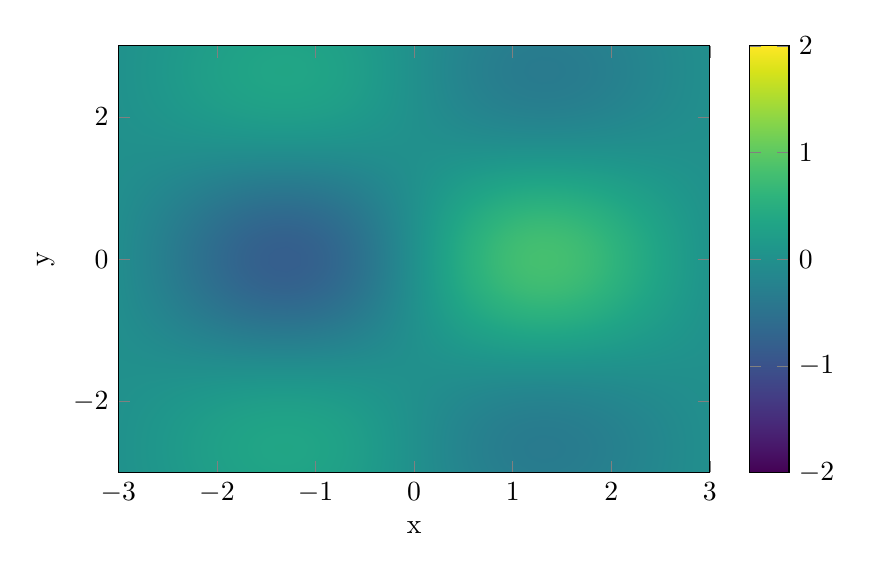
\begin{tikzpicture}
    \begin{axis}[
        width=0.75\textwidth,
        height=7cm,
        xlabel={x},
        ylabel={y},
        view={0}{90},
        colorbar,
        colormap/viridis,
        point meta min=-2,
        point meta max=2,
    ]
        \addplot3[
            surf,
            shader=interp,
            domain=-3:3,
            domain y=-3:3,
            samples=50,
        ] {sin(deg(x))*cos(deg(y))*exp(-0.1*(x*x+y*y))};
    \end{axis}
    \end{tikzpicture}
    \caption{Contour plot of $f(x,y) = \sin(x)\cos(y)\,e^{-0.1(x^2+y^2)}$.}
    \label{fig:contour}
\end{figure}

% =====================================================
\section{3D Surface Plot}
\label{sec:surface}
% =====================================================

A parametric 3D surface with lighting effects.

\begin{figure}[htbp]
    \centering
    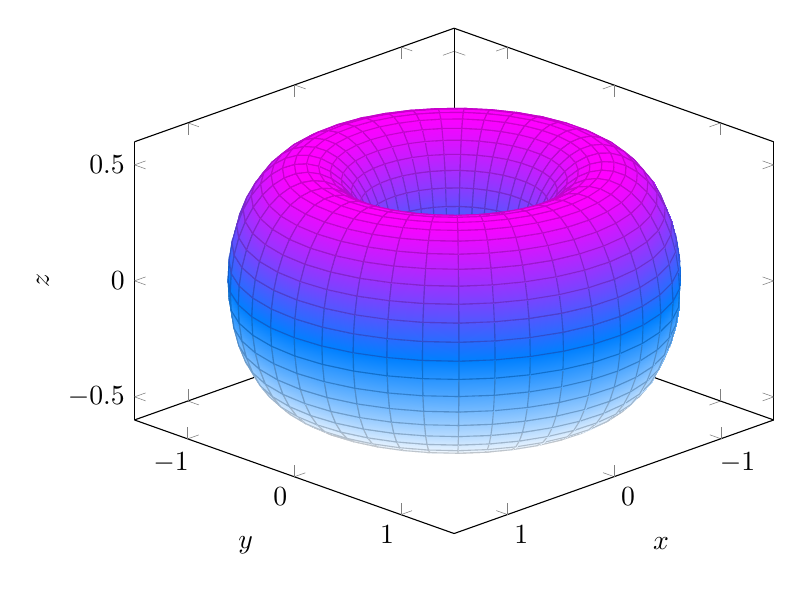
\begin{tikzpicture}
    \begin{axis}[
        width=0.8\textwidth,
        height=8cm,
        xlabel={$x$},
        ylabel={$y$},
        zlabel={$z$},
        view={135}{30},
        colormap/cool,
        z buffer=sort,
    ]
        \addplot3[
            surf,
            shader=faceted interp,
            domain=0:360,
            domain y=0:360,
            samples=40,
            samples y=40,
        ] (
            {cos(x)*(1+0.5*cos(y))},
            {sin(x)*(1+0.5*cos(y))},
            {0.5*sin(y)}
        );
    \end{axis}
    \end{tikzpicture}
    \caption{Torus surface parameterized by $(x,y) \mapsto (\cos x(1+0.5\cos y),\;\sin x(1+0.5\cos y),\;0.5\sin y)$.}
    \label{fig:surface}
\end{figure}

% =====================================================
\section{Circuit Diagram}
\label{sec:circuit}
% =====================================================

An electronic circuit using the \texttt{circuitikz} package.

\begin{figure}[htbp]
    \centering
    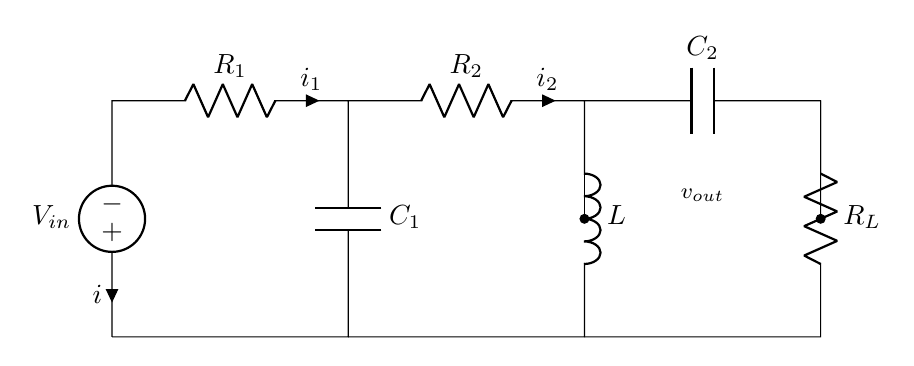
\begin{tikzpicture}[american]
        \draw (0,0)
            to[V, l=$V_{in}$, i=$i$] (0,3)
            to[R, l=$R_1$, i=$i_1$] (3,3)
            to[C, l=$C_1$] (3,0)
            -- (0,0);
        \draw (3,3)
            to[R, l=$R_2$, i=$i_2$] (6,3)
            to[L, l=$L$] (6,0)
            -- (3,0);
        \draw (6,3)
            to[C, l=$C_2$] (9,3)
            to[R, l=$R_L$] (9,0)
            -- (6,0);
        \draw (9,3) -- (9,2) to[short, -*] (9,1.5);
        \draw (6,3) -- (6,2) to[short, -*] (6,1.5);
        \node at (7.5,1.8) {\footnotesize $v_{out}$};
    \end{tikzpicture}
    \caption{Multi-stage RLC filter circuit with input and output voltage labels.}
    \label{fig:circuit}
\end{figure}

% =====================================================
\section{Gantt Chart}
\label{sec:gantt}
% =====================================================

A project timeline Gantt chart with task dependencies.

\begin{figure}[htbp]
    \centering
    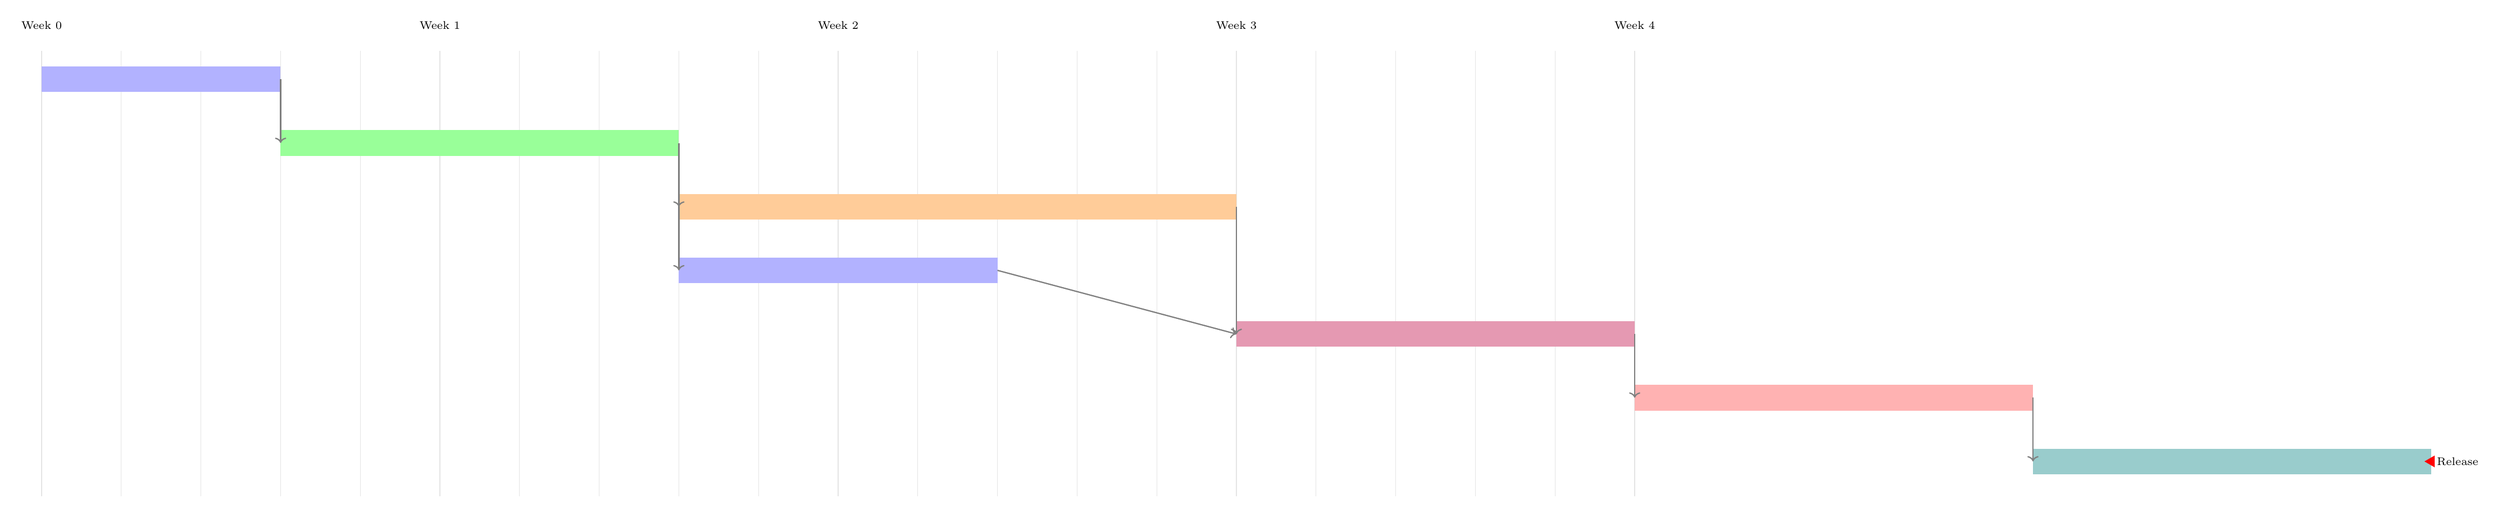
\begin{tikzpicture}[
        x=0.35cm, y=0.7cm,
        bar/.style={fill=blue!50, rounded corners=1pt},
        milestone/.style={fill=red, regular polygon, regular polygon sides=3,
            inner sep=1.5pt, rotate=90},
        dep/.style={->, thick, gray},
    ]
        % Grid
        \foreach \w in {0,...,20} {
            \draw[gray!20] (\w*5, -0.5) -- (\w*5, -14.5);
        }
        \foreach \w in {0,...,4} {
            \node[above, font=\scriptsize] at (\w*25, 0) {Week \w};
        }

        % Task bars
        \fill[blue!30] (0, -1) rectangle (15, -1.8) node[midway, font=\footnotesize] {Requirements};
        \fill[green!40] (15, -3) rectangle (40, -3.8) node[midway, font=\footnotesize] {Design};
        \fill[orange!40] (40, -5) rectangle (75, -5.8) node[midway, font=\footnotesize] {Implementation};
        \fill[blue!30] (40, -7) rectangle (60, -7.8) node[midway, font=\footnotesize] {Unit Tests};
        \fill[purple!40] (75, -9) rectangle (100, -9.8) node[midway, font=\footnotesize] {Integration};
        \fill[red!30] (100, -11) rectangle (125, -11.8) node[midway, font=\footnotesize] {User Testing};
        \fill[teal!40] (125, -13) rectangle (150, -13.8) node[midway, font=\footnotesize] {Deployment};

        % Dependencies
        \draw[dep] (15, -1.4) -- (15, -3.4);
        \draw[dep] (40, -3.4) -- (40, -5.4);
        \draw[dep] (40, -3.4) -- (40, -7.4);
        \draw[dep] (60, -7.4) -- (75, -9.4);
        \draw[dep] (75, -5.4) -- (75, -9.4);
        \draw[dep] (100, -9.4) -- (100, -11.4);
        \draw[dep] (125, -11.4) -- (125, -13.4);

        % Milestone
        \node[milestone] at (150, -13.4) {};
        \node[right, font=\scriptsize] at (150, -13.4) {Release};
    \end{tikzpicture}
    \caption{Project Gantt chart showing task schedule and dependencies.}
    \label{fig:gantt}
\end{figure}

% =====================================================
\section{Organizational Chart}
\label{sec:org-chart}
% =====================================================

A corporate hierarchy organizational chart.

\begin{figure}[htbp]
    \centering
    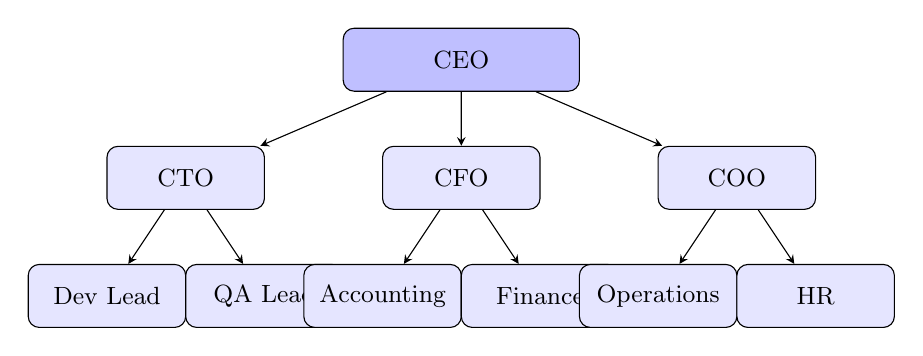
\begin{tikzpicture}[
        level 1/.style={sibling distance=3.5cm},
        level 2/.style={sibling distance=2cm},
        every node/.style={draw, rounded corners, fill=blue!10,
            minimum width=2cm, minimum height=0.8cm, font=\small,
            text centered},
        edge from parent/.style={draw, ->, >=stealth},
        grow=down,
    ]
        \node[fill=blue!25, minimum width=3cm] {CEO}
            child { node {CTO}
                child { node {Dev Lead} }
                child { node {QA Lead} }
            }
            child { node {CFO}
                child { node {Accounting} }
                child { node {Finance} }
            }
            child { node {COO}
                child { node {Operations} }
                child { node {HR} }
            };
    \end{tikzpicture}
    \caption{Organizational hierarchy chart.}
    \label{fig:org-chart}
\end{figure}

% =====================================================
\section{Mind Map}
\label{sec:mind-map}
% =====================================================

A radial mind map for knowledge organization.

\begin{figure}[htbp]
    \centering
    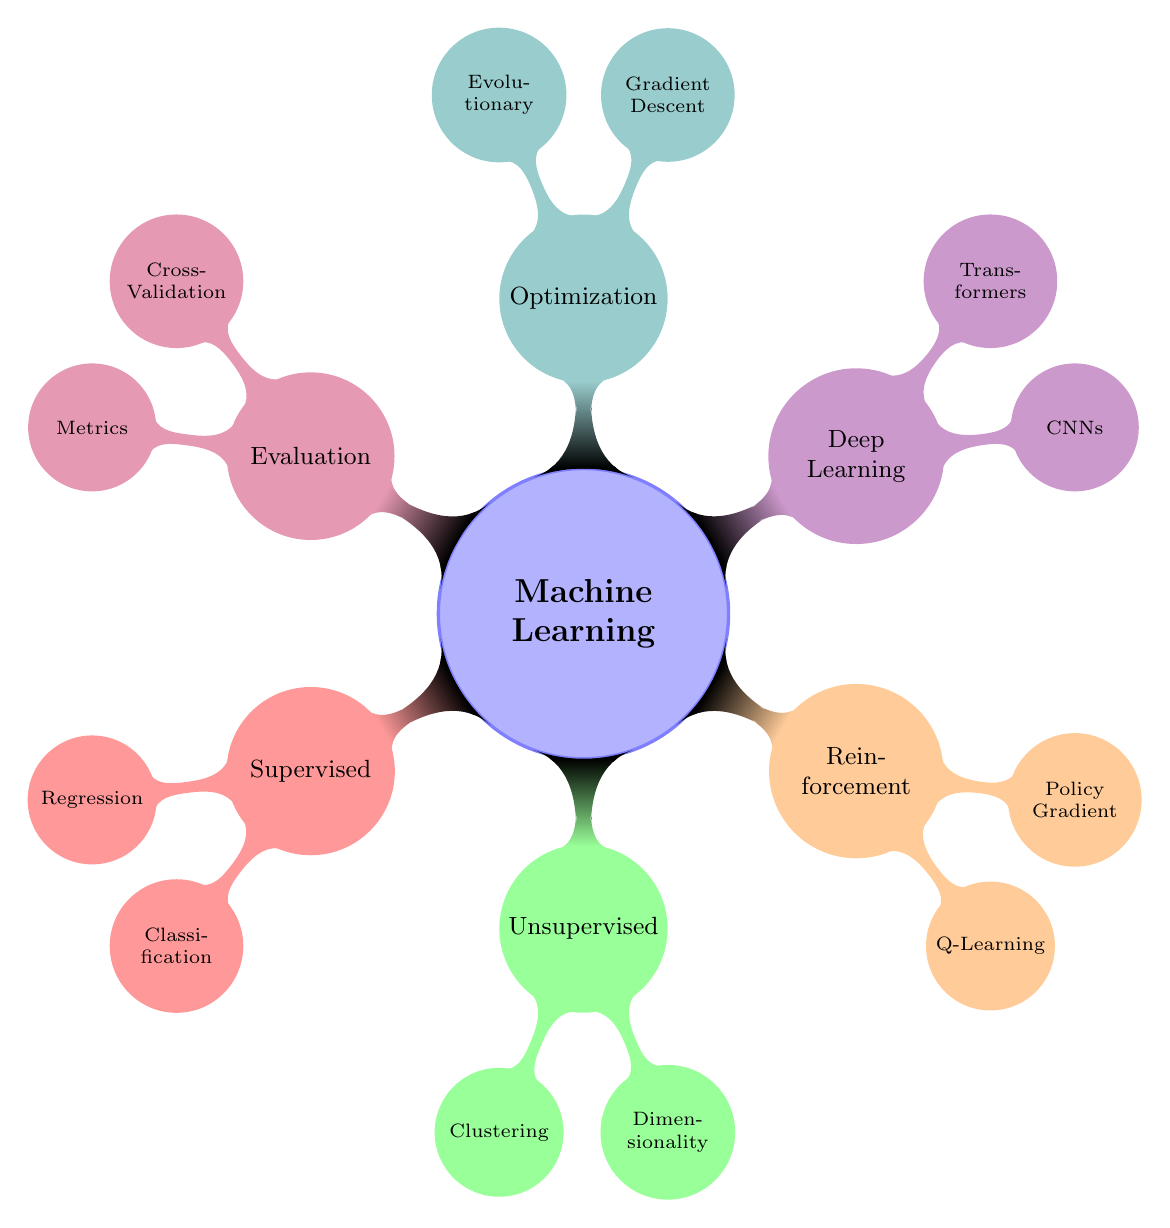
\begin{tikzpicture}[
        mindmap,
        grow cyclic,
        every node/.style={concept, execute at begin node=\hskip0pt},
        root concept/.append style={
            concept color=blue!50, fill=blue!30,
            font=\large\bfseries, minimum size=3cm,
        },
        level 1 concept/.append style={
            font=\small, minimum size=2cm, level distance=4cm,
            sibling angle=60,
        },
        level 2/.append style={
            font=\scriptsize, minimum size=1.5cm,
            level distance=2.8cm, sibling angle=45,
        },
    ]
        \node[text width=3cm, align=center, root concept] {Machine Learning}
            child[concept color=red!40] { node {Supervised}
                child { node {Regression} }
                child { node {Classification} }
            }
            child[concept color=green!40] { node {Unsupervised}
                child { node {Clustering} }
                child { node {Dimensionality} }
            }
            child[concept color=orange!40] { node {Reinforcement}
                child { node {Q-Learning} }
                child { node {Policy Gradient} }
            }
            child[concept color=violet!40] { node {Deep Learning}
                child { node {CNNs} }
                child { node {Transformers} }
            }
            child[concept color=teal!40] { node {Optimization}
                child { node {Gradient Descent} }
                child { node {Evolutionary} }
            }
            child[concept color=purple!40] { node {Evaluation}
                child { node {Cross-Validation} }
                child { node {Metrics} }
            };
    \end{tikzpicture}
    \caption{Mind map of machine learning sub-disciplines.}
    \label{fig:mind-map}
\end{figure}

% =====================================================
\section{Timeline}
\label{sec:timeline}
% =====================================================

A horizontal timeline marking key events.

\begin{figure}[htbp]
    \centering
    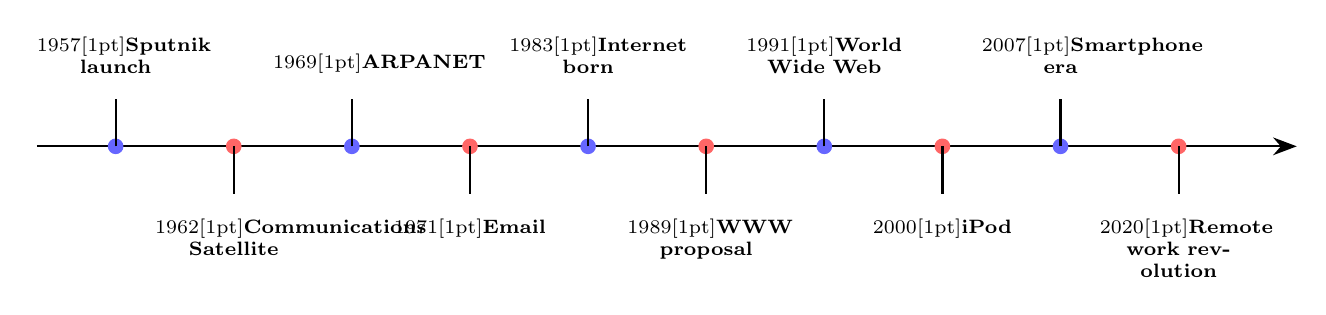
\begin{tikzpicture}[
        event/.style={circle, fill=blue!60, inner sep=2pt, minimum size=5pt},
        label/.style={font=\scriptsize, text width=2cm, align=center},
    ]
        % Main line
        \draw[thick, -{Stealth[length=3mm]}] (0,0) -- (16,0);

        % Events above
        \foreach \x/\year/\text in {
            1/1957/Sputnik launch,
            4/1969/ARPANET,
            7/1983/Internet born,
            10/1991/World Wide Web,
            13/2007/Smartphone era
        } {
            \node[event] at (\x, 0) {};
            \draw[thick] (\x, 0) -- (\x, 0.6);
            \node[text width=3cm, align=center, label, above] at (\x, 0.8) {\year [1pt]\textbf{\text}};
        }

        % Events below
        \foreach \x/\year/\text in {
            2.5/1962/Communications Satellite,
            5.5/1971/Email,
            8.5/1989/WWW proposal,
            11.5/2000/iPod,
            14.5/2020/Remote work revolution
        } {
            \node[event, fill=red!60] at (\x, 0) {};
            \draw[thick] (\x, 0) -- (\x, -0.6);
            \node[text width=3cm, align=center, label, below] at (\x, -0.8) {\year [1pt]\textbf{\text}};
        }
    \end{tikzpicture}
    \caption{Timeline of major technology milestones.}
    \label{fig:timeline}
\end{figure}

% =====================================================
\section{Sankey Diagram}
\label{sec:sankey}
% =====================================================

A flow visualization showing energy distribution.

\begin{figure}[htbp]
    \centering
    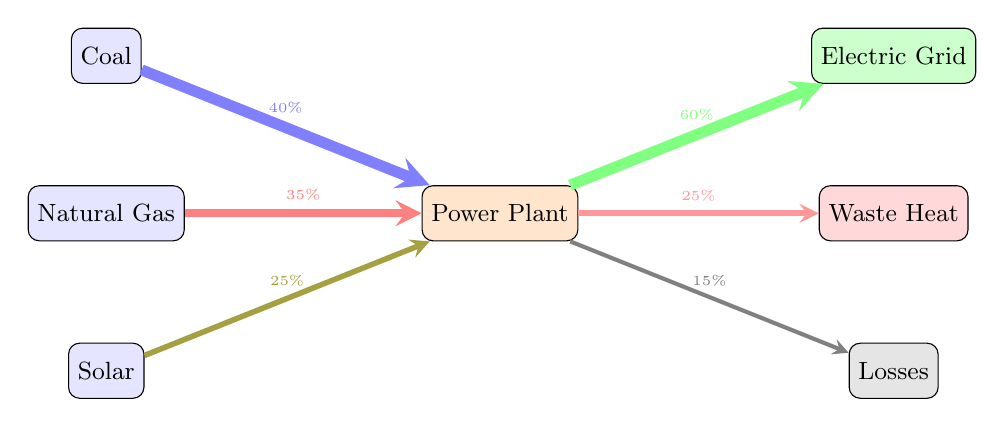
\begin{tikzpicture}[
        node style/.style={draw, rounded corners, fill=blue!10,
            minimum height=0.7cm, font=\small, text centered},
        flow/.style={->, >=stealth, thick},
    ]
        % Source nodes
        \node[node style] (coal) at (0, 2) {Coal};
        \node[node style] (gas) at (0, 0) {Natural Gas};
        \node[node style] (solar) at (0, -2) {Solar};

        % Intermediate
        \node[node style, fill=orange!20] (power) at (5, 0) {Power Plant};

        % Output nodes
        \node[node style, fill=green!20] (grid) at (10, 2) {Electric Grid};
        \node[node style, fill=red!15] (heat) at (10, 0) {Waste Heat};
        \node[node style, fill=gray!20] (loss) at (10, -2) {Losses};

        % Flows (thick arrows with varying widths)
        \draw[flow, line width=4pt, blue!50] (coal) -- node[above, font=\tiny] {40\%} (power);
        \draw[flow, line width=3pt, red!50] (gas) -- node[above, font=\tiny] {35\%} (power);
        \draw[flow, line width=2pt, yellow!60!black] (solar) -- node[above, font=\tiny] {25\%} (power);

        \draw[flow, line width=4pt, green!50] (power) -- node[above, font=\tiny] {60\%} (grid);
        \draw[flow, line width=2pt, red!40] (power) -- node[above, font=\tiny] {25\%} (heat);
        \draw[flow, line width=1.5pt, gray] (power) -- node[above, font=\tiny] {15\%} (loss);
    \end{tikzpicture}
    \caption{Energy Sankey diagram: sources to grid with losses.}
    \label{fig:sankey}
\end{figure}

% =====================================================
\section{Geometric Constructions}
\label{sec:geometric}
% =====================================================

Compass-and-straightedge construction of a perpendicular bisector.

\begin{figure}[htbp]
    \centering
    \begin{tikzpicture}[
        >=stealth,
        line width=0.8pt,
    ]
        % Line segment AB
        \draw[thick] (-3,0) coordinate(A) -- (3,0) coordinate(B);
        \node[below left] at (A) {$A$};
        \node[below right] at (B) {$B$};

        % Midpoint
        \fill (0,0) coordinate(M) circle (1.5pt);
        \node[below] at (M) {$M$};

        % Arc from A
        \draw[blue, thin, dashed] (A) ++(60:3.5) arc (60:120:3.5);
        \draw[blue, thin, dashed] (B) ++(60:3.5) arc (60:-0:3.5);

        % Construction arcs
        \draw[red, thin] (A) ++(60:3.2) arc (60:120:3.2) coordinate[pos=0] (P1);
        \draw[red, thin] (A) ++(120:3.2) arc (120:180:3.2) coordinate[pos=0] (P2);
        \draw[red, thin] (B) ++(60:3.2) arc (60:0:3.2) coordinate[pos=0] (Q1);
        \draw[red, thin] (B) ++(0:3.2) arc (0:-60:3.2) coordinate[pos=0] (Q2);

        % Intersection points (perpendicular bisector)
        \coordinate (top) at (0, 2.8);
        \coordinate (bot) at (0, -2.8);

        % Perpendicular line
        \draw[thick, green!60!black] (top) -- (bot);
        \node[left] at (top) {$\ell$};

        % Right angle marker
        \draw[thick] (0,0.3) -- (0.3,0.3) -- (0.3,0);

        % Construction marks
        \foreach \pt in {P1,P2,Q1,Q2} {
            \fill[red] (\pt) circle (1pt);
        }

        % Labels
        \node[above left, font=\scriptsize, blue] at (-2.5, 2.5) {Arcs from $A$};
        \node[above right, font=\scriptsize, blue] at (2.5, 2.5) {Arcs from $B$};
    \end{tikzpicture}
    \caption{Compass-and-straightedge construction of the perpendicular bisector of segment $AB$.}
    \label{fig:geometric}
\end{figure}

% =====================================================
\section{Data Flow Diagram}
\label{sec:data-flow}
% =====================================================

A system data flow diagram showing data movement between processes.

\begin{figure}[htbp]
    \centering
    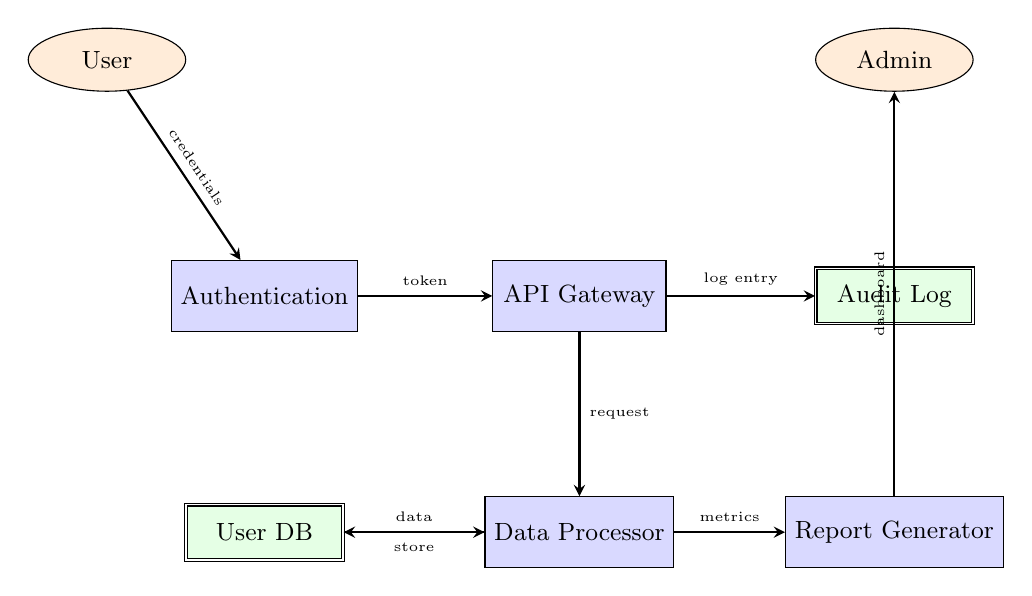
\begin{tikzpicture}[
        process/.style={rectangle, draw, fill=blue!15, minimum width=2.2cm,
            minimum height=0.9cm, text centered, font=\small},
        datastore/.style={rectangle, draw, fill=green!10, minimum width=2cm,
            minimum height=0.7cm, text centered, font=\small, double},
        external/.style={ellipse, draw, fill=orange!15, minimum width=2cm,
            minimum height=0.8cm, text centered, font=\small},
        flow/.style={->, >=stealth, thick},
    ]
        % External entities
        \node[external] (user) at (0, 3) {User};
        \node[external] (admin) at (10, 3) {Admin};

        % Processes
        \node[process] (auth) at (2, 0) {Authentication};
        \node[process] (api) at (6, 0) {API Gateway};
        \node[process] (proc) at (6, -3) {Data Processor};
        \node[process] (report) at (10, -3) {Report Generator};

        % Data stores
        \node[datastore] (db) at (2, -3) {User DB};
        \node[datastore] (log) at (10, 0) {Audit Log};

        % Flows
        \draw[flow] (user) -- node[above, sloped, font=\tiny] {credentials} (auth);
        \draw[flow] (auth) -- node[above, font=\tiny] {token} (api);
        \draw[flow] (api) -- node[right, font=\tiny] {request} (proc);
        \draw[flow] (proc) -- node[below, font=\tiny] {store} (db);
        \draw[flow] (db) -- node[above, sloped, font=\tiny] {data} (proc);
        \draw[flow] (proc) -- node[above, font=\tiny] {metrics} (report);
        \draw[flow] (report) -- node[above, sloped, font=\tiny] {dashboard} (admin);
        \draw[flow] (api) -- node[above, sloped, font=\tiny] {log entry} (log);
    \end{tikzpicture}
    \caption{Data flow diagram for a web application backend.}
    \label{fig:data-flow}
\end{figure}

% =====================================================
\section{UML Class Diagram}
\label{sec:class-diagram}
% =====================================================

A UML class diagram with inheritance and associations.

\begin{figure}[htbp]
    \centering
    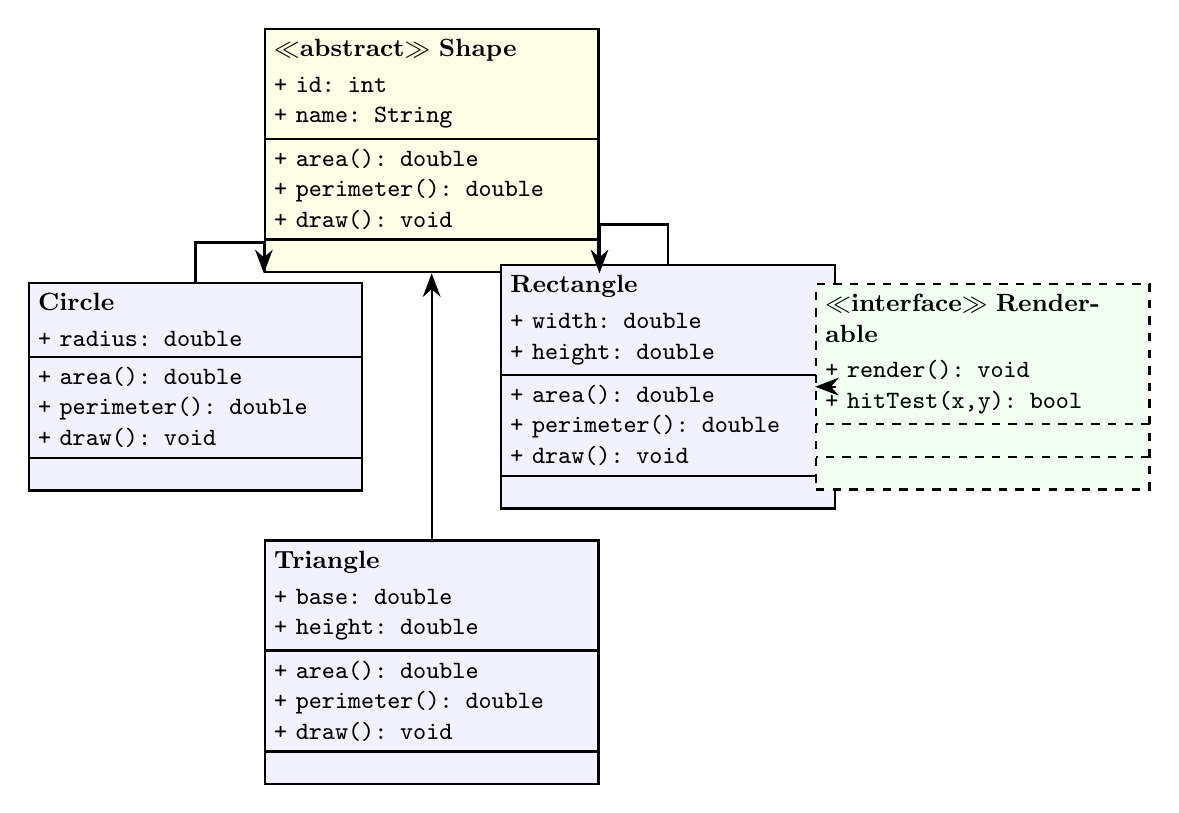
\begin{tikzpicture}[
        class/.style={rectangle split, rectangle split parts=3,
            draw, thick, fill=blue!5, text width=4cm,
            font=\small, align=left},
        interface/.style={class, fill=green!5, dashed},
        rel/.style={-{Stealth[length=3mm]}, thick},
        assoc/.style={-{Stealth[length=3mm]}, thick, gray},
    ]
        % Abstract class
        \node[class, fill=yellow!10, text width=4cm, align=left] (shape) at (0, 3) {
            \textbf{$\ll$abstract$\gg$ Shape}\\[2pt]
            \texttt{+ id: int}\\
            \texttt{+ name: String}
            \nodepart{two}
            \texttt{+ area(): double}\\
            \texttt{+ perimeter(): double}\\
            \texttt{+ draw(): void}
        };

        % Concrete classes
        \node[class] (circle) at (-3, 0) {
            \textbf{Circle}\\[2pt]
            \texttt{+ radius: double}
            \nodepart{two}
            \texttt{+ area(): double}\\
            \texttt{+ perimeter(): double}\\
            \texttt{+ draw(): void}
        };
        \node[class] (rect) at (3, 0) {
            \textbf{Rectangle}\\[2pt]
            \texttt{+ width: double}\\
            \texttt{+ height: double}
            \nodepart{two}
            \texttt{+ area(): double}\\
            \texttt{+ perimeter(): double}\\
            \texttt{+ draw(): void}
        };
        \node[class] (tri) at (0, -3.5) {
            \textbf{Triangle}\\[2pt]
            \texttt{+ base: double}\\
            \texttt{+ height: double}
            \nodepart{two}
            \texttt{+ area(): double}\\
            \texttt{+ perimeter(): double}\\
            \texttt{+ draw(): void}
        };

        % Inheritance
        \draw[rel] (circle.north) -- ++(0,0.5) -| (shape.south west);
        \draw[rel] (rect.north) -- ++(0,0.5) -| (shape.south east);
        \draw[rel] (tri.north) -- (shape.south);

        % Interface
        \node[interface] (renderable) at (7, 0) {
            \textbf{$\ll$interface$\gg$ Renderable}\\[2pt]
            \texttt{+ render(): void}\\
            \texttt{+ hitTest(x,y): bool}
        };

        % Realization
        \draw[rel, dashed] (rect.east) -- (renderable.west);
    \end{tikzpicture}
    \caption{UML class diagram: Shape hierarchy with a \texttt{Renderable} interface.}
    \label{fig:class-diagram}
\end{figure}

% =====================================================
\section{Directed Graph}
\label{sec:directed-graph}
% =====================================================

A weighted directed graph with labeled edges.

\begin{figure}[htbp]
    \centering
    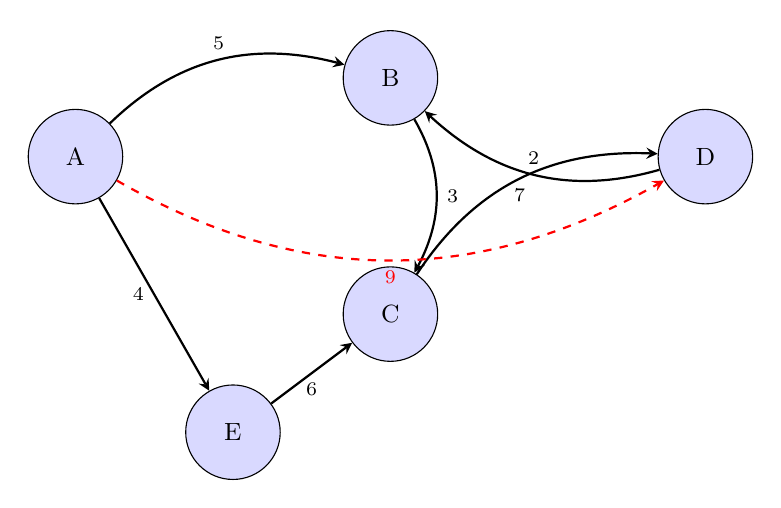
\begin{tikzpicture}[
        vertex/.style={circle, draw, fill=blue!15, minimum size=12mm,
            inner sep=0pt, font=\small},
        every edge/.style={draw, ->, >=stealth, thick},
    ]
        \node[vertex] (a) at (0, 2) {A};
        \node[vertex] (b) at (4, 3) {B};
        \node[vertex] (c) at (4, 0) {C};
        \node[vertex] (d) at (8, 2) {D};
        \node[vertex] (e) at (2, -1.5) {E};

        \draw[->, thick] (a) edge[bend left] node[above, font=\scriptsize] {5} (b);
        \draw[->, thick] (b) edge[bend left] node[right, font=\scriptsize] {3} (c);
        \draw[->, thick] (c) edge[bend left] node[below, font=\scriptsize] {7} (d);
        \draw[->, thick] (d) edge[bend left] node[above, font=\scriptsize] {2} (b);
        \draw[->, thick] (a) edge node[left, font=\scriptsize] {4} (e);
        \draw[->, thick] (e) edge node[below, font=\scriptsize] {6} (c);
        \draw[->, thick, dashed, red] (a) edge[bend right] node[below, font=\scriptsize] {9} (d);
    \end{tikzpicture}
    \caption{Weighted directed graph. Dashed red edge indicates a shortcut.}
    \label{fig:directed-graph}
\end{figure}

% =====================================================
\section{Polar Plot}
\label{sec:polar}
% =====================================================

A polar coordinate plot showing a rose curve.

\begin{figure}[htbp]
    \centering
    \begin{tikzpicture}
    \begin{polaraxis}[
        width=0.65\textwidth,
        height=0.65\textwidth,
        grid=major,
        legend style={at={(1.1,0.5)}, anchor=west, font=\small},
    ]
        \addplot[blue, thick, domain=0:360, samples=200]
            {3*cos(2*x)};
        \addplot[red, thick, domain=0:360, samples=200]
            {2.5*sin(3*x)};
        \legend{Four-petal rose, Three-petal rose}
    \end{polaraxis}
    \end{tikzpicture}
    \caption{Polar plot of rose curves $r = 3\cos(2\theta)$ and $r = 2.5\sin(3\theta)$.}
    \label{fig:polar}
\end{figure}

% =====================================================
\section{Conclusion}
\label{sec:conclusion}
% =====================================================

This gallery demonstrates the breadth of diagram types achievable with TikZ and
pgfplots. From flowcharts and neural networks to UML diagrams and polar plots,
the combination of these packages provides a comprehensive toolkit for
scientific and technical illustration. Each diagram is self-contained and can be
adapted for publications, presentations, or technical documentation.

\end{document}
